\documentclass[10.5pt,a4paper]{article}
\usepackage[a4paper,left=2.6cm,right=2.6cm,top=2.6cm,bottom=2.5cm]{geometry}
\usepackage{fontspec}
\usepackage{xeCJK}
\setCJKmainfont{AR PL SungtiL GB}[AutoFakeBold=2.5]
\setCJKsansfont{AR PL SungtiL GB}[AutoFakeBold=2.5]
\usepackage{xcolor,graphicx,booktabs,array,amsmath,titlesec,enumitem,caption,float,indentfirst}
\titleformat{\section}{\bfseries\large}{\thesection}{.7em}{}
\titleformat{\subsection}{\bfseries\normalsize}{\thesubsection}{.6em}{}
\titlespacing*{\section}{0pt}{1.4em}{.6em}\titlespacing*{\subsection}{0pt}{1em}{.4em}
\pagestyle{plain}
\renewcommand{\figurename}{图}\renewcommand{\tablename}{表}
\captionsetup{font=small,labelfont=bf,labelsep=quad,skip=4pt}
\setlist[itemize]{leftmargin=1.6em,itemsep=1pt,topsep=2pt,parsep=0pt}
\setlist[enumerate]{leftmargin=1.8em,itemsep=1pt,topsep=2pt,parsep=0pt}
\setlength{\parindent}{2em}\setlength{\parskip}{0pt}\linespread{1.25}
\renewcommand{\arraystretch}{1.15}
\newcommand{\bv}[1]{\textbf{#1}}
\begin{document}

\begin{center}
{\LARGE\bfseries 扩散先验稀疏观测同化\par}\vspace{.5em}
{\large Rayleigh--B\'enard 对流实验汇报\par}
\end{center}
\vspace{.3em}

\begin{center}\textbf{摘\quad 要}\end{center}
\begingroup\small\leftskip=2em\rightskip=2em
在仅有 1\% 稀疏观测、数值模式存在模型误差（Rayleigh 数失配）的条件下，比较三种同化方案：A 背景场与稀疏观测联合同化（扩散先验 + DPS），B 稀疏观测直接重建，C 集合卡尔曼滤波（EnKF）。3 个测试 case、每帧进观测的结果表明，A 的未观测点 RMSE 为 0.0135，B 为 0.0171，C 为 0.0196，A 较 B、C 分别降低 21\% 和 31\%；该优势在 3 个 case 中 2 个显著、1 个持平。原始分析场的速度散度上扩散模型大于 EnKF，但经求解器重启所用的流函数投影后三者无明显差异。初值噪声（至 40\% 参考标准差）使纯预报误差增大约 24\%，同化后几乎不受影响。长时间（400 个循环）下扩散模型方法稳定在约 0.011，EnKF 约 0.019。
\par\endgroup

\section{实验设置}
\subsection{控制方程、数据与时间尺度}
研究对象为二维 Boussinesq Rayleigh--B\'enard 对流，状态为浮力 $b$ 与速度 $\mathbf u=(u_x,u_z)$：
\begin{equation}
\nabla\!\cdot\!\mathbf u=0,\qquad \partial_t b-\kappa\nabla^2 b=-\mathbf u\!\cdot\!\nabla b,\qquad \partial_t\mathbf u-\nu\nabla^2\mathbf u+\nabla p-b\,\mathbf e_z=-\mathbf u\!\cdot\!\nabla\mathbf u,
\end{equation}
其中 $\kappa=(\mathrm{Ra}\,\mathrm{Pr})^{-1/2}$，$\nu=(\mathrm{Ra}/\mathrm{Pr})^{-1/2}$。$x$ 方向周期（$L_x=3$），$z$ 方向为上下壁面（$L_z=1$），边界条件为 $b(0)=1$、$b(L_z)=0$、壁面无滑移。真实流动取 $\mathrm{Ra}=1\times10^{5}$、$\mathrm{Pr}=1$，用 Dedalus v3 求解（$x$ 方向 Fourier、$z$ 方向 Chebyshev，网格 $72\times24$，时间步长 $\mathrm{d}t=0.01$）。

数据集含 200 条轨迹，弃去前 120 帧瞬态后每条保留 100 帧，按 160/20/20 划分训练、验证、测试集，本文使用测试 case 0--2，验证 case 仅用于调参。1 帧对应 35 个求解器步（0.35 个时间单位），100 帧共 3500 步（35 个时间单位）。

\subsection{模型误差、观测与评价指标}
背景模型同为 Dedalus，但 Rayleigh 数取 $5\times10^{4}$（真值 $1\times10^{5}$），这是唯一的模型误差来源，由求解器自身产生，不人为加噪。观测为真值的 1\% 随机格点（1728 个格点中的 17 个，位置固定），三个通道同时观测，无噪声；主对比中每帧进一次观测。

评价指标为未观测格点上的均方根误差（RMSE，三通道合并）。方程平衡用相对散度 $\|\nabla\!\cdot\!\mathbf u\|/\|\nabla\mathbf u\|$ 衡量，导数用 Fourier--Chebyshev 谱方法计算，真值约为 $3.4\times10^{-5}$。所有方法的参数均在验证 case 上选定，在测试 case 上比较；DPS 与 EnKF 均关闭硬观测覆盖。

\section{同化方法与对照方案}
先验为无条件扩散模型（VP-cosine 噪声调度，U-Net，基础通道数 16，训练 200 个 epoch），只学习流场快照的分布，不接触观测、背景场和时间。同化逐帧循环（图~\ref{fig:wf}）：上一帧分析场经 Dedalus 预报（先做流函数投影后重启，推进 35 步）得到背景场；背景场与当前帧观测一并作为似然引导项进入扩散后验采样（DPS，100 步，8 个样本取均值），采样从纯噪声开始。第 0 帧没有背景场，只用观测。

\begin{figure}[htbp]\centering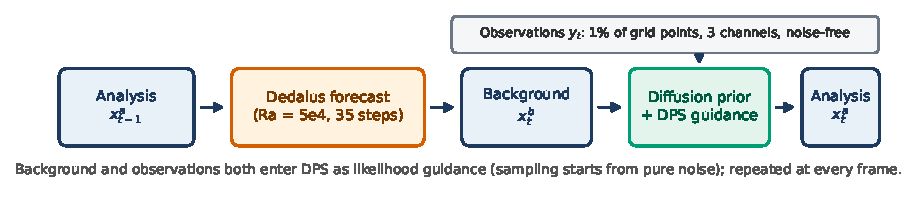
\includegraphics[width=\linewidth]{report_fig/workflow.pdf}\caption{逐帧循环同化流程（方案 A）。}\label{fig:wf}\end{figure}

\begin{table}[htbp]\centering\small\caption{三个对照方案}
\begin{tabular}{@{}c>{\raggedright\arraybackslash}p{3.6cm}>{\raggedright\arraybackslash}p{3.1cm}>{\raggedright\arraybackslash}p{5.2cm}@{}}\toprule
方案 & 方法 & 背景场 & 主要参数（验证 case 上选定）\\ \midrule
A & 背景场 + 稀疏观测联合同化 & Dedalus 预报 & DPS：$b_\mathrm{std}=0.3$，rate $=2$，$o_\mathrm{std}=0.05$ \\
B & 稀疏观测直接重建 & 无 & DPS：$o_\mathrm{std}=0.025$，rate $=2$；每帧独立采样 \\
C & 随机 EnKF & 成员由 Dedalus 预报 & 20 成员；膨胀 2.5；Gaspari--Cohn 局地化 $1.5(x)\times1.2(z)$；$R=0.01$ \\ \bottomrule\end{tabular}\end{table}

EnKF 的更新式为 $\mathbf x^a-\mathbf x^f=\mathbf P^f\mathbf H^{\!\top}(\mathbf H\mathbf P^f\mathbf H^{\!\top}+\mathbf R)^{-1}[\mathbf y-H(\mathbf x^f)]$，采用扰动观测、逐观测点顺序同化，分析场取集合均值。其初始集合以 DPS 第 0 帧的分析场为中心，因此比较的是同一初始分析之后的循环；散度在预报重启之前测量。

\section{结果}
\subsection{重建误差}
表~\ref{tab:res} 给出每帧进观测时三个方案的未观测点 RMSE。A 的合并误差最低，为 0.0135，较 B 降低 21\%，较 C 降低 31\%；分通道看，A 在 $b$、$u_x$、$u_z$ 上均最低。分 case 看，A 在 case 1、2 上明显更低，在 case 0 上与 B 基本持平（0.0152 对 0.0149）。EnKF 的误差集中在 $b$ 通道（0.0256）。每 3 帧进观测时，A 为 0.0145，EnKF（膨胀加局地化）为 0.0195，仅膨胀为 0.0214，无膨胀无局地化为 0.0319（几乎不吸收观测，误差随时间上涨）。

\begin{table}[htbp]\centering\small\caption{未观测点 RMSE（每帧进观测，3 个测试 case $\times$ 100 帧；粗体为最小值）}\label{tab:res}
\begin{tabular}{@{}lccccccc@{}}\toprule
方案 & $b$ & $u_x$ & $u_z$ & 合并 & case 0 & case 1 & case 2 \\ \midrule
A\ \ 背景场 + 观测 & \bv{0.0136} & \bv{0.0139} & \bv{0.0127} & \bv{0.0135} & 0.0152 & \bv{0.0133} & \bv{0.0119} \\
B\ \ 仅观测 & 0.0168 & 0.0177 & 0.0167 & 0.0171 & \bv{0.0149} & 0.0171 & 0.0193 \\
C\ \ EnKF & 0.0256 & 0.0169 & 0.0143 & 0.0196 & 0.0177 & 0.0211 & 0.0201 \\ \bottomrule\end{tabular}\end{table}

\begin{figure}[htbp]\centering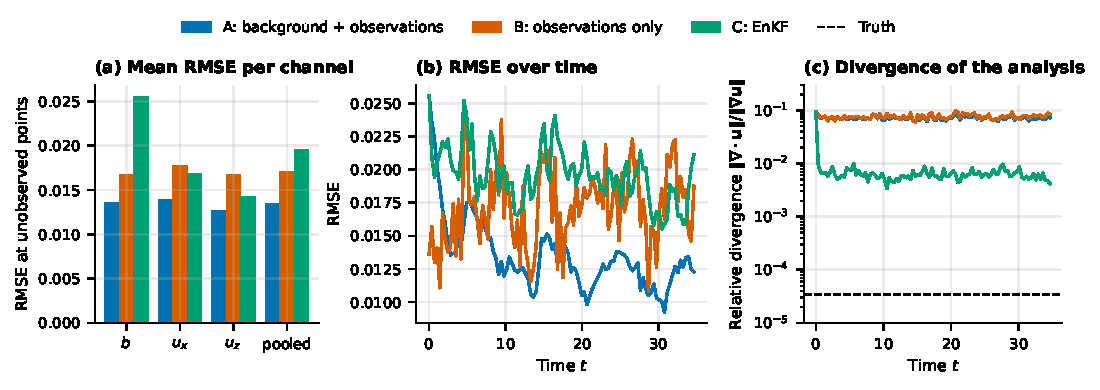
\includegraphics[width=\linewidth]{report_fig/unified.pdf}\caption{三个方案的误差与散度（每帧进观测，3 个测试 case）。}\end{figure}

\subsection{背景场的作用}
图~\ref{fig:fusion} 比较有背景场（A）与无背景场（B）的逐帧误差。背景场平均有益，但并不稳定：case 1、2 显著受益，case 0 持平；循环初期（约前 6 个时间单位），上一步分析尚不准，预报出的背景场反而拖累结果，A 不如 B。此外 B 每帧独立采样、没有时间连续性，A 的优势有一部分来自求解器带来的时间连续性，而非背景场精度本身。

\begin{figure}[htbp]\centering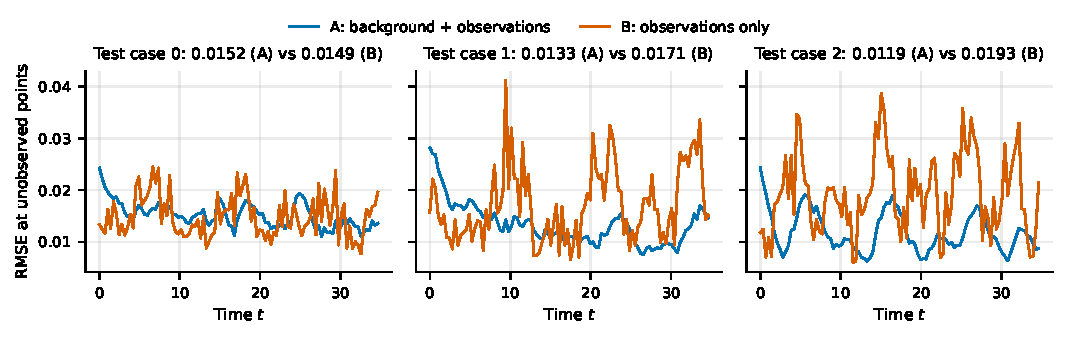
\includegraphics[width=\linewidth]{report_fig/fusion.pdf}\caption{A 与 B 的逐帧 RMSE，标题给出各 case 的平均值。}\label{fig:fusion}\end{figure}

\subsection{流场对比}
图~\ref{fig:field} 给出测试 case 1 第 60 帧的浮力场：A 的绝对误差整体最小，B 的残差更大且分布更广，C 在局部出现较大的误差斑块。

\begin{figure}[htbp]\centering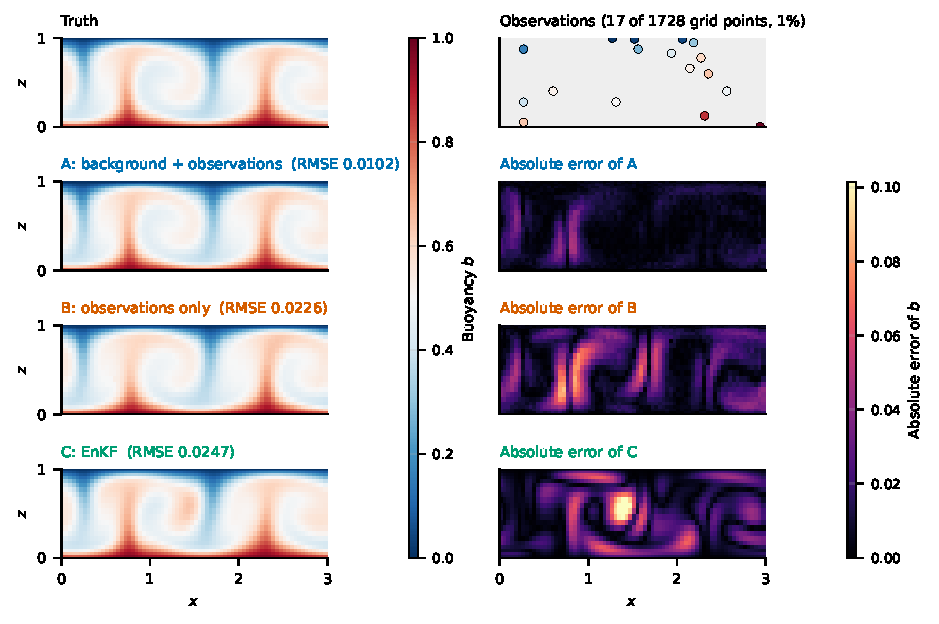
\includegraphics[width=.95\linewidth]{report_fig/field.pdf}\caption{测试 case 1、第 60 帧的浮力 $b$：左列为真值与 A/B/C 的分析场，右列为观测位置与三个方案的绝对误差（色标统一）。}\label{fig:field}\end{figure}

\subsection{方程平衡}
表~\ref{tab:div} 给出分析场的相对散度。原始分析场上，A、B 约 0.07，C 约 0.006，真值约 $3.4\times10^{-5}$，扩散模型的分析场不严格满足不可压缩。但每帧预报前求解器重启会做流函数投影，原始分析场的不平衡不会累积；经同样的投影后，三者的散度均约 0.008，贴近对真值做同样投影的下限（0.0079），差异不明显，且投影几乎不改变速度对真值的误差。这说明原始散度偏大主要来自小尺度毛刺被求导放大（给真值速度加 0.6\% 白噪声即可使散度升至 0.06），该解释在 3 个 case、102 帧上验证。

不带局地化的 EnKF 散度约 $10^{-5}$，低于真值，但这并非同化质量所致：成员均由求解器预报、近似无散度，其线性组合亦然（纯预报约 $9\times10^{-6}$）；局地化对不同位置赋予不同权重，破坏了这一性质，散度升至 $10^{-3}$ 量级。

\begin{table}[htbp]\centering\small\caption{分析场的相对散度与速度误差（投影列为 3 个 case、每 3 帧取样的均值）}\label{tab:div}
\begin{tabular}{@{}lcccc@{}}\toprule
方案 & 原始分析场 & 投影后 & 速度 RMSE（投影前） & 速度 RMSE（投影后） \\ \midrule
A\ \ 背景场 + 观测 & 0.0706 & 0.0084 & 0.01348 & 0.01335 \\
B\ \ 仅观测 & 0.0752 & 0.0084 & 0.01744 & 0.01690 \\
C\ \ EnKF & 0.0060 & 0.0075 & 0.01562 & 0.01564 \\ \midrule
真值经同样投影 & $3.4\times10^{-5}$ & 0.0079 & --- & --- \\ \bottomrule\end{tabular}\end{table}

\subsection{初值噪声}
在 $t=0$ 的真值上叠加平滑噪声：$b$ 的噪声乘壁面包络（壁面处为零）；速度由流函数噪声求导得到，因而无散度且壁面为零，$u_x$、$u_z$ 共用一个缩放系数。噪声幅度为水平乘参考标准差（$b$ 去掉 $x$ 平均后约 0.097，$u_x$、$u_z$ 约 0.166 和 0.169），水平取 0 至 40\%，每档 3 个样本，在测试 case 0 上比较。结果见表~\ref{tab:noise} 与图~\ref{fig:noise}：40\% 噪声使不同化的纯预报全程平均误差增大 24\%，每帧同化的 DPS 几乎不变。需要说明的是，到末 10 帧纯预报已因模型误差涨至约 0.052，初值噪声的影响被淹没，因此该实验的区分度偏弱。

\begin{figure}[htbp]\centering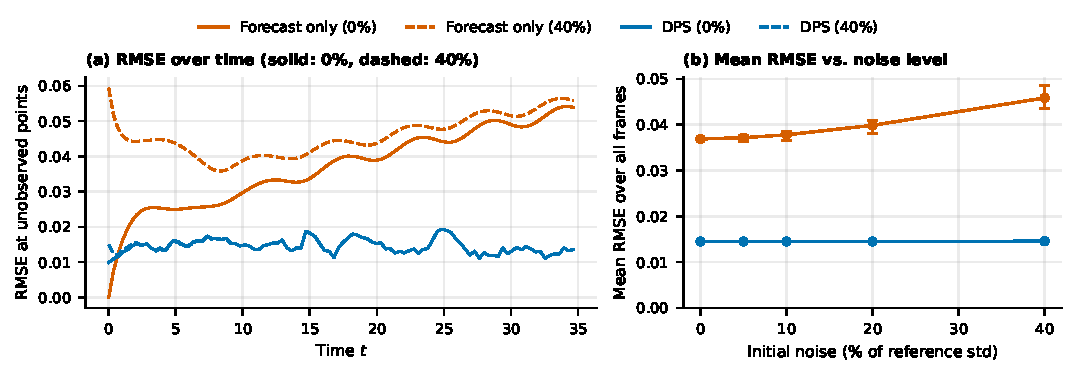
\includegraphics[width=\linewidth]{report_fig/noise.pdf}\caption{$t=0$ 叠加不同水平噪声的影响（误差线为 3 个噪声样本的范围）。}\label{fig:noise}\end{figure}

\begin{table}[htbp]\centering\small\caption{初值噪声对未观测点 RMSE 的影响（测试 case 0）}\label{tab:noise}
\begin{tabular}{@{}lccccc@{}}\toprule
方案 & 无噪声 & 40\% 噪声 & 变化 & 末 10 帧（无噪声） & 末 10 帧（40\%） \\ \midrule
纯预报 & 0.0369 & 0.0458 & +24\% & 0.0522 & 0.0553 \\
DPS 每帧观测 & 0.0145 & 0.0146 & +0\% & 0.0128 & 0.0128 \\
DPS 每 3 帧观测 & 0.0148 & 0.0151 & +2\% & 0.0134 & 0.0134 \\ \bottomrule\end{tabular}\end{table}

\subsection{长时间表现}
将 3 条测试轨迹重新积分到 520 帧，取其中 400 个循环（约 140 个时间单位），每 3 帧进观测。DPS 约在 100 帧后收敛至约 0.011，EnKF 全程约 0.019（全程平均 0.0120 对 0.0190），3 个 case 均为 DPS 更低（图~\ref{fig:long}）。真值在该区间已是统计稳态（动能约 0.0276，$b$ 标准差约 0.257，帧间变化约 0.0127），但流场仍在演化。误差走平是否源于模型误差注入与观测修正的平衡，尚未验证（可改变 Rayleigh 数失配量，观察平线高度是否随之变化）。

\begin{figure}[htbp]\centering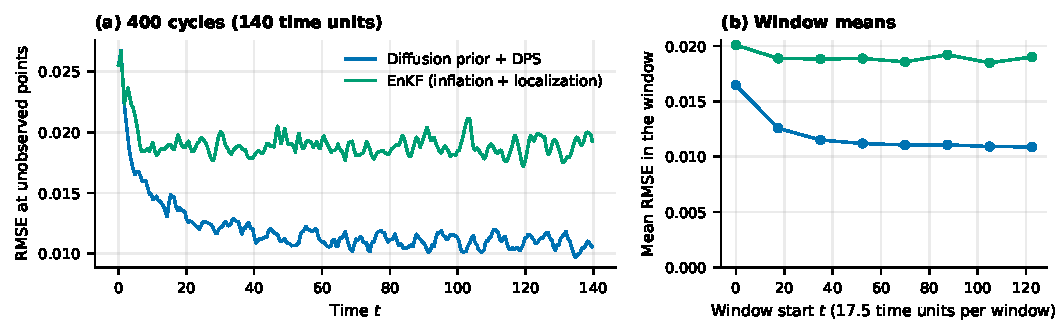
\includegraphics[width=\linewidth]{report_fig/long.pdf}\caption{400 个循环的 RMSE（a）与每 17.5 个时间单位窗口内的平均 RMSE（b）。}\label{fig:long}\end{figure}

\section{结论}
\begin{enumerate}
\item 背景场与稀疏观测联合同化（A）的未观测点 RMSE 最低（0.0135），较稀疏观测直接重建降低 21\%，较 EnKF 降低 31\%；对 B 的优势在 3 个 case 中 2 个显著、1 个持平，且循环初期背景场不利。
\item 原始分析场的散度上扩散模型明显大于 EnKF；经求解器重启所用的流函数投影后三者无明显差异。
\item 初值噪声（至 40\%）使纯预报误差增大约 24\%，同化后几乎不受影响。
\item 长时间下 A 稳定在约 0.011，EnKF 约 0.019。
\end{enumerate}

\section{局限}
结果来自 3 个测试 case、单个随机种子，初值噪声实验仅用测试 case 0。实验为孪生设定：观测无噪声、三通道同时观测、模型误差仅为 Rayleigh 数失配一种，较真实场景容易。EnKF 只用了 20 个成员（未测 40 及以上），更新式按通用形式实现，待与任务给定公式核对。散度偏大的解释仅在 102 帧样本上验证。后续工作包括多种子与更多 case、EnKF 增加成员、改变失配量与观测比例、观测加噪。

\end{document}
